% This LaTeX was auto-generated from MATLAB code.
% To make changes, update the MATLAB code and export to LaTeX again.

\documentclass{article}

\usepackage[utf8]{inputenc}
\usepackage[T1]{fontenc}
\usepackage{lmodern}
\usepackage{graphicx}
\usepackage{color}
\usepackage{listings}
\usepackage{hyperref}
\usepackage{amsmath}
\usepackage{amsfonts}
\usepackage{epstopdf}
\usepackage{matlab}

\sloppy
\epstopdfsetup{outdir=./}
\graphicspath{ {./hw1_images/} }

\begin{document}

\matlabtitle{Home work 1                                               (15-Jan-2019)}

\begin{matlabcode}
t = randn(1000000,1)*pi;

x = sin(t);
y = sin(2*t);
\end{matlabcode}


\matlabheading{Histograms}

\begin{matlabcode}
histogram(x);
title('histogram of x');
\end{matlabcode}
\begin{center}
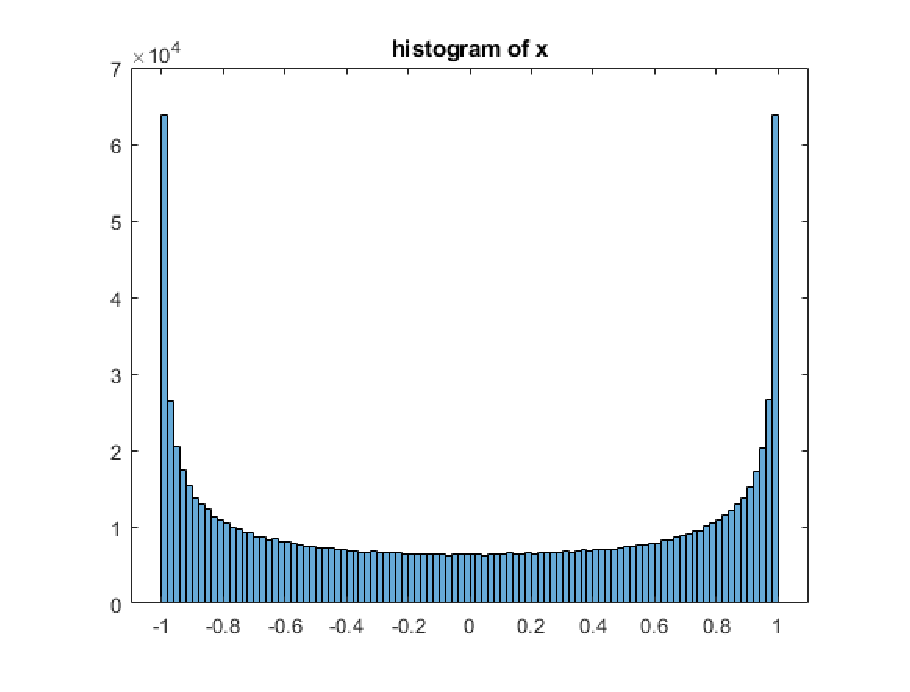
\includegraphics[width=\maxwidth{56.196688409433015em}]{figure_0}
\end{center}
\begin{matlabcode}
histogram(y);
title('histogram of y')
\end{matlabcode}
\begin{center}
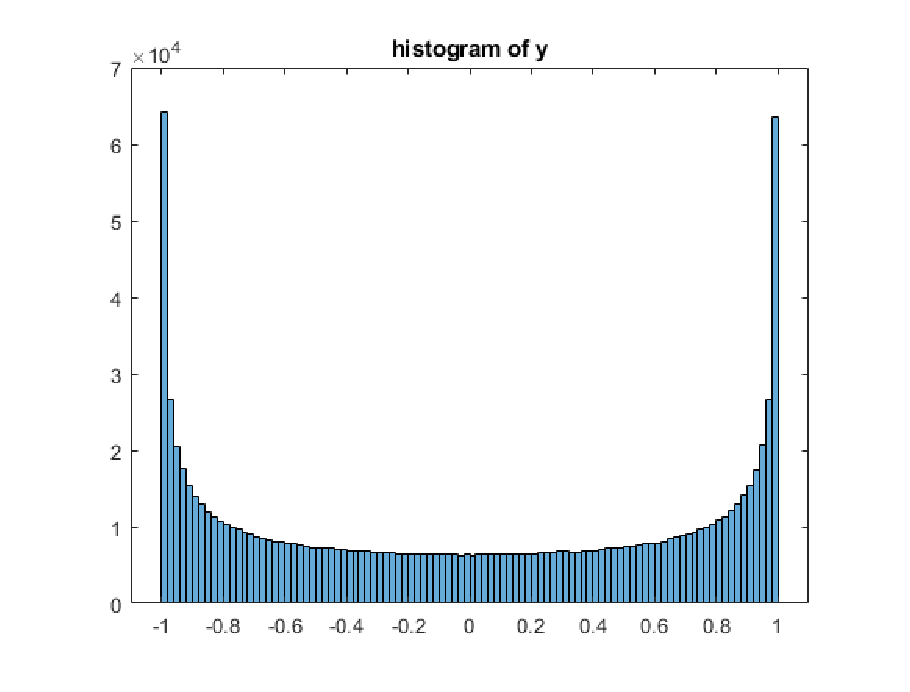
\includegraphics[width=\maxwidth{56.196688409433015em}]{figure_1}
\end{center}


\matlabheading{Probability density density}

\begin{matlabcode}
[f_x,xi] = ksdensity(x);
[f_y,yi] = ksdensity(y);

plot(xi, f_x, 'r', yi, f_y, '--g');
legend({'x', 'y'}, 'Location','best');
title('pdf of x and y');
\end{matlabcode}
\begin{center}
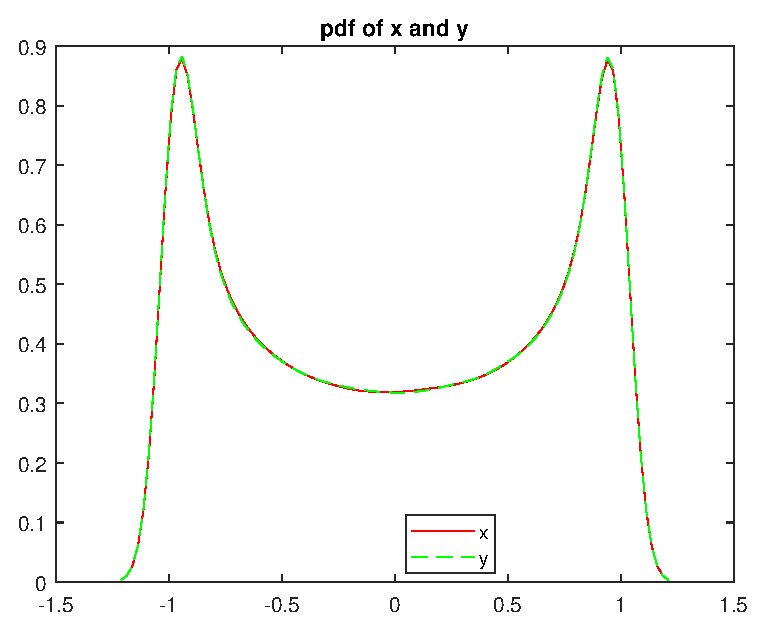
\includegraphics[width=\maxwidth{56.196688409433015em}]{figure_2}
\end{center}


\matlabheading{Joint Histogram}

\begin{matlabcode}
hist3([x,y]);
xlabel('x');
ylabel('y');
\end{matlabcode}
\begin{center}
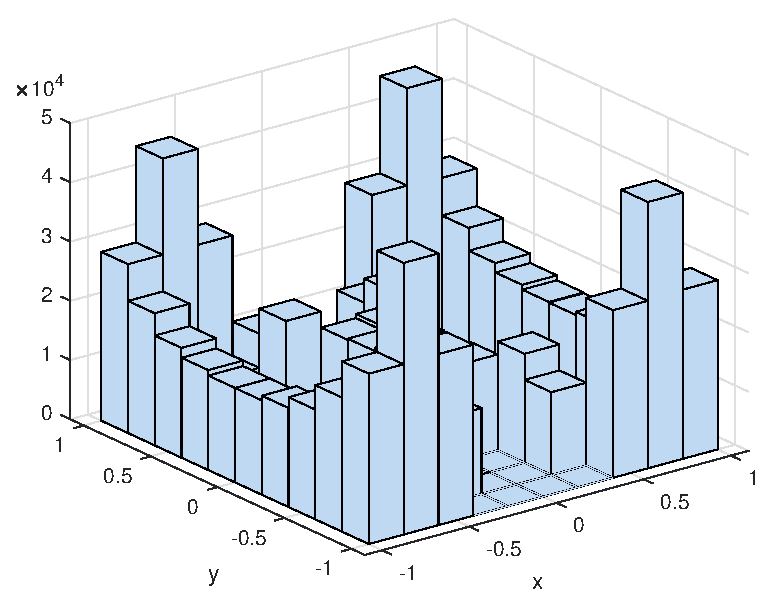
\includegraphics[width=\maxwidth{56.196688409433015em}]{figure_3}
\end{center}


\matlabheading{Joint Probability function}

\begin{matlabcode}
ksdensity([x,y]);
title('Joint probability distribution');
\end{matlabcode}
\begin{center}
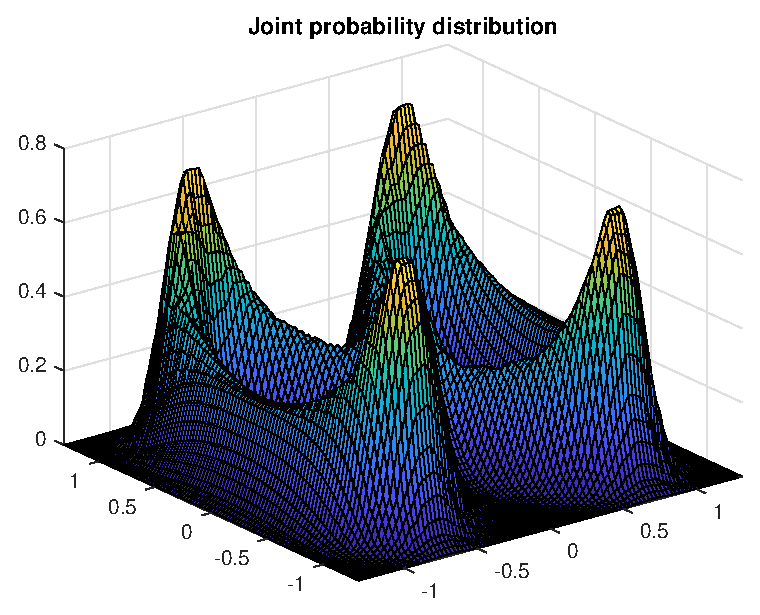
\includegraphics[width=\maxwidth{56.196688409433015em}]{figure_4}
\end{center}

\end{document}
